\section{Loading data}
\paragraph{}
For our following experiments, we will use the following textures:
\begin{figure}[h]
    \centering
    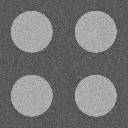
\includegraphics[scale=0.6]{rdf-2-classes-texture-0.png}
    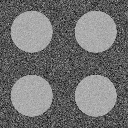
\includegraphics[scale=0.6]{rdf-2-classes-texture-1.png}
    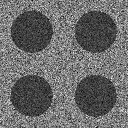
\includegraphics[scale=0.6]{rdf-2-classes-texture-2.png}
    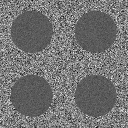
\includegraphics[scale=0.6]{rdf-2-classes-texture-3.png}
    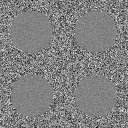
\includegraphics[scale=0.6]{rdf-2-classes-texture-4.png}
    \caption{Images to experiment on}
\end{figure}

\paragraph{}
Our reference image (having a clear difference between objects and background) is the following:
\begin{figure}[h]
    \centering
    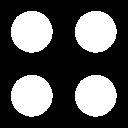
\includegraphics[scale=0.6]{rdf-masque-ronds.png}
    \caption{Reference image}
    \label{fig-reference-image}
\end{figure}

\paragraph{}
These will be loaded and converted to gray images:
\begin{lstlisting}[language=R, caption=Loading images]
    rdfReadGreyImage <- function (nom) {
        image <- readImage (nom)
        if (length (dim (image)) == 2) {
            image
        } else {
            channel (image, 'red')
        }
    }
\end{lstlisting}

\clearpage

\section{Gray levels}
\subsection{Gray values histograms}
\paragraph{}
A first good step would be taking a look at how the gray values are distributed. We can use a \emph{histogram} for this.
\begin{lstlisting}[language=R, caption=Creating histograms of gray values]
    buildHistogram <- function (nom, nbins){
        image <- rdfReadGreyImage (nom)
        h <- hist (as.vector (image), breaks = seq (0, 1, 1 / nbins), main = nom)
    }
\end{lstlisting}

\begin{figure}[h]
    \centering
    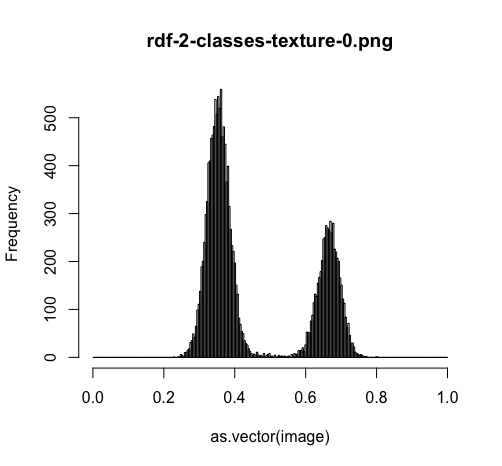
\includegraphics[width=\textwidth/3]{gray_values_0.png}
    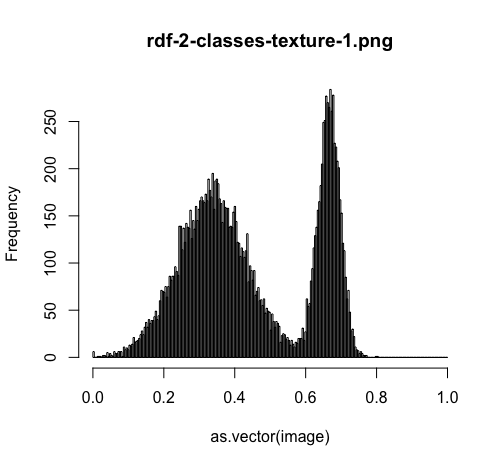
\includegraphics[width=\textwidth/3]{gray_values_1.png}
    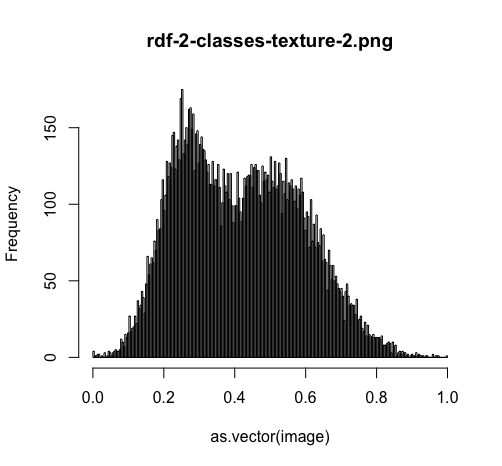
\includegraphics[width=\textwidth/3]{gray_values_2.png}
    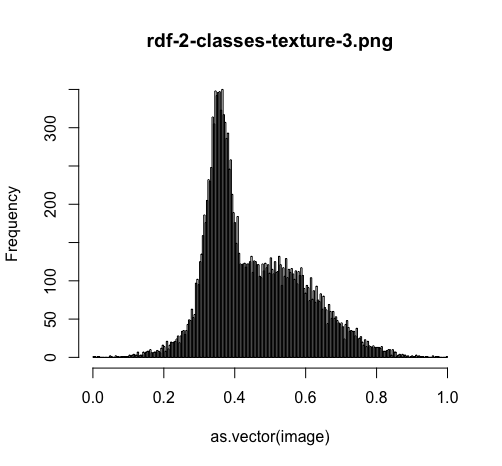
\includegraphics[width=\textwidth/3]{gray_values_3.png}
    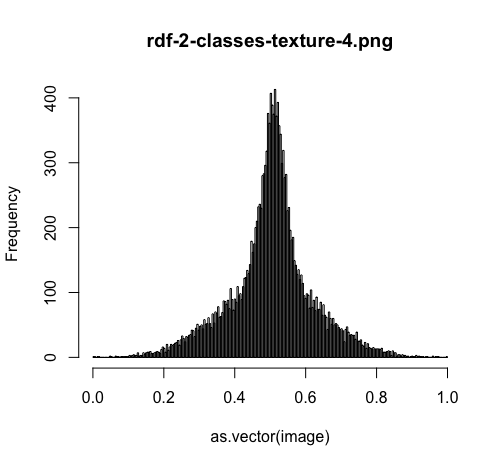
\includegraphics[width=\textwidth/3]{gray_values_4.png}
    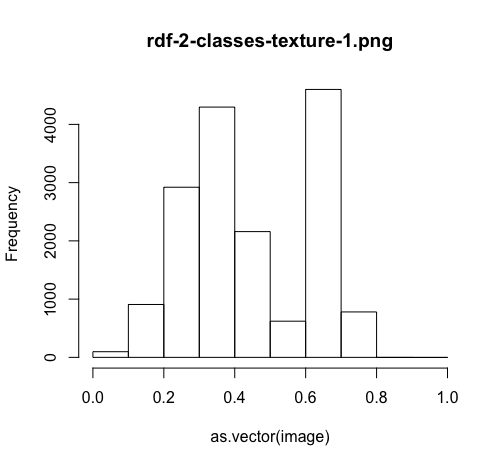
\includegraphics[width=\textwidth/3]{histogram_10bins.png}
    \caption{Histograms of gray values}
    \label{fig-histograms}
\end{figure}

\paragraph{}
Since each pixel can have a gray value from $0$ to $255$, we therefore have a total number of $256$ values, so that is going to be our number of \emph{bins} for the histogram.
If we were to use, for example, only $10$ bins, that would give the number of pixels with gray values between $[0, 0.1)$, $[0.1, 0.2)$ and so on, as it can be seen in the last image \ref{fig-histograms}.

\subsection{Thresholding based on gray values}
\paragraph{}
\label{experiment-thresholding}
Based on the histograms above \ref{fig-histograms}, we may have our first attempt at a simple form of \emph{image segmentation}.
By picking the gray value at which (as explained in the figure below), we can classify the pixels on the left as being part of objects, and the others on the right as being part of the background.
\cite{lille_rdf_course}
\begin{figure}[h]
    \centering
    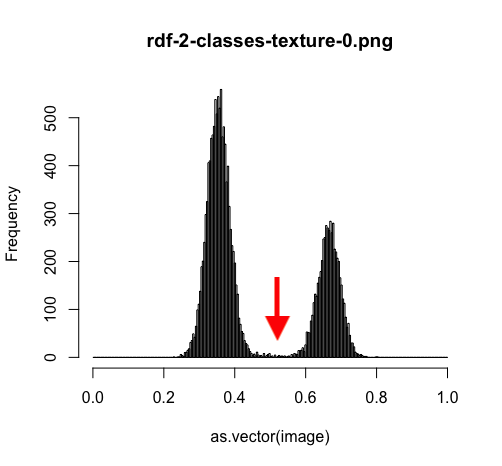
\includegraphics[scale=0.5]{threshold_explanation.png}
    \caption{Choosing the threshold}
    \label{fig-threshold-explanation}
\end{figure}

\begin{lstlisting}[language=R, caption=Segmenting based on the gray threshold]
    buildBinaryImage <- function(nom, threshold){
        image <- rdfReadGreyImage (nom)
        binaire <- (image - threshold) >= 0
        # a "trick" to make the error calculation more precise
        bin_1 = sum(binaire)
        bin_0 = dim(binaire)[1] * dim(binaire)[2] - bin_1
        if (bin_0 < bin_1)
            binaire = 1 - binaire
        
        # reference image
        reference <- rdfReadGreyImage ("rdf-masque-ronds.png")
        # results
        error = sum(binaire != reference) / (dim(reference)[1] * dim(reference)[2])
        error = round (error, 4) * 100
        info <- sprintf("%s\nthreshold=%s\nerror=%s%%", nom, threshold, error)
        if (interactive()){
            display (binaire, "image binaire", method="raster", all=TRUE)
            legend(x=0.5, y=dim(binaire)[2]/2, info, bg = "lightgreen", box.col = "lightgreen", yjust=0.5)
        }
    }
\end{lstlisting}

\paragraph{}
Observation: in the code above, we consider that the majority of pixels are for objects.
Therefore, if in our segmentation it's the opposite way, we reverse the image (lines 5-8) so we have a more precise error \footnote{The error represents the percent of missclassified pixels, relative to the reference image} calculation.

\clearpage

\paragraph{}
Taking a look at the results, we realise it was not incorrect to call this a \emph{simple} form of segmentation.
It's rather effective to reach about the same results as our reference image \ref{fig-reference-image} for the first 2 textures, having a low error.
However, for the last 2, we don't have a clear ``valley'' \ref{fig-threshold-explanation} in the histogram that we can use as our threshold.
For example, the histogram of the last texture resembles a Gaussian distribution, therefore the gray values are evenly distributed relative to their center: $\mu\approx0.5$.
\paragraph{}
As a result, we receive an error of about $50\%$ for the last texture when trying to somewhat resemble the reference image.
Our lowest error will be achieved by setting the threshold to either $0$ or $1$, but that will not help us at all.

\begin{figure}[h]
    \centering
    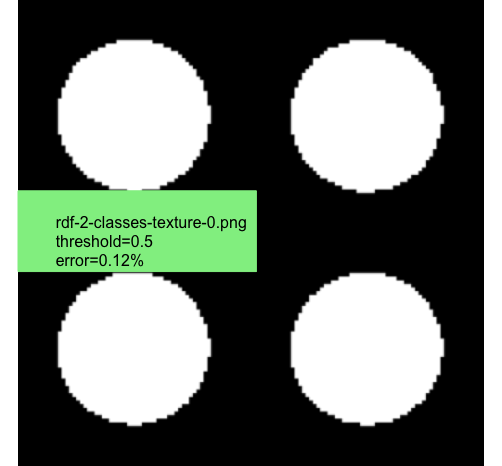
\includegraphics[width=\textwidth/3]{gray_thresholding_0.png}
    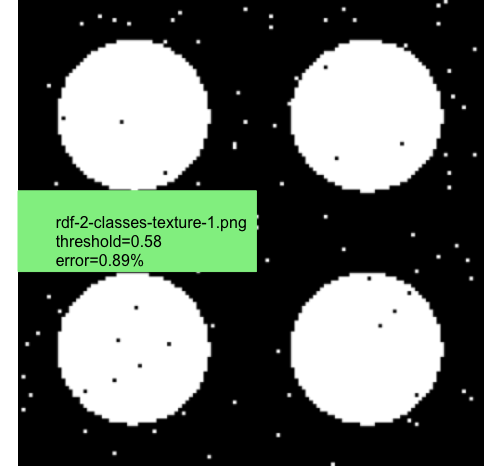
\includegraphics[width=\textwidth/3]{gray_thresholding_1.png}
    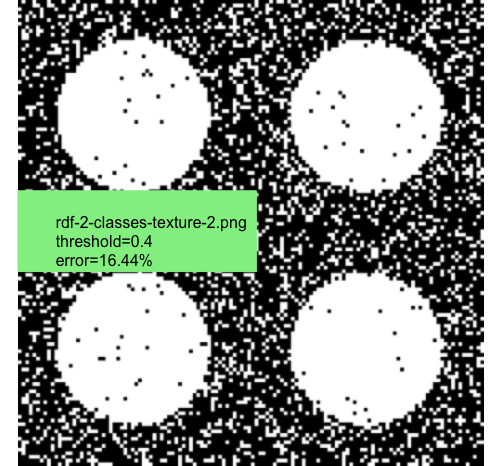
\includegraphics[width=\textwidth/3]{gray_thresholding_2.png}
    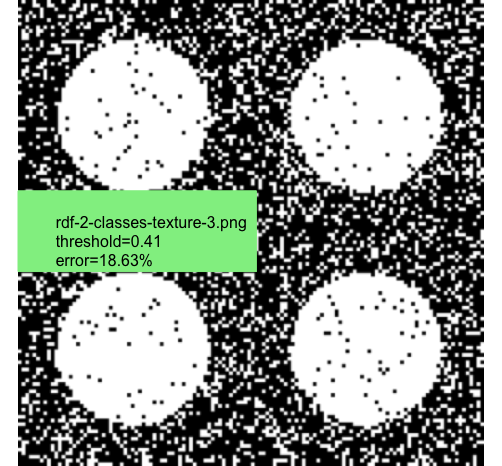
\includegraphics[width=\textwidth/3]{gray_thresholding_3.png}
    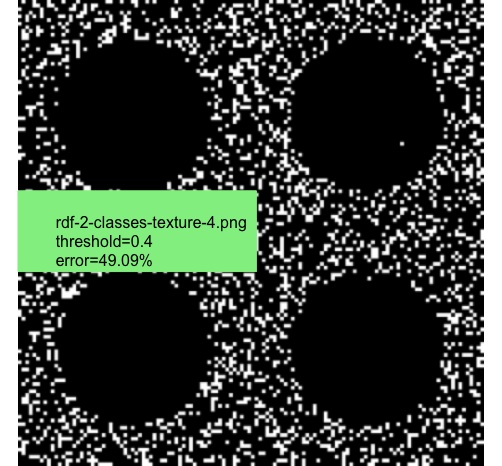
\includegraphics[width=\textwidth/3]{gray_thresholding_4_1.png}
    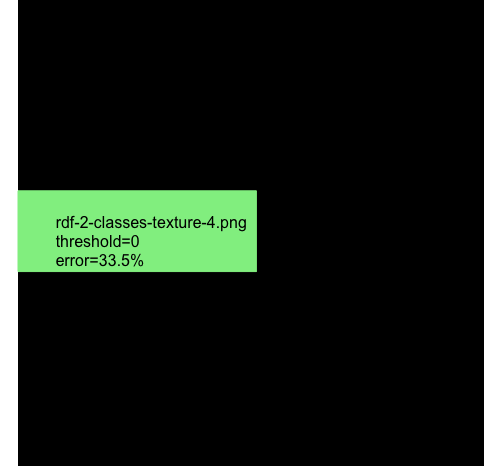
\includegraphics[width=\textwidth/3]{gray_thresholding_4_2.png}
    \caption{Image segmentation based on gray threshold}
\end{figure}

\paragraph{}
We can conclude this experiment by saying that this method will not suffice, especially for ``noisy'' textures, as seen above.
Even for the simple textures we still have some missclassified pixels, as it's hard (or often times impossible) to get the right threshold for a perfect segmentation.
It is intuitive that the single white pixels (for example for the second texture) surrounded by black pixels should also be part of the background, so next we'll focus on trying to use a pixel's neighbours to gain more information.

\clearpage

\section{Texture levels}
\subsection{Calculating texture levels}
\paragraph{}
We can define a pixel's \emph{texture level} as being the standard deviation of the gray levels for the pixels located in a square neighborhood.
Intuitively, a big value for the standard deviation will mean that the nearby pixels have very different gray values.
We could therefore say that the current pixel is a \emph{border} between an object and the background.
\paragraph{}
To calculate this, we first select the \emph{neighbourhood size} we want to work with.
That will represent the number of nearby pixels we'll take into consideration when calculating the standard deviation.
A neighbourhood size of $2$ will give us a square of $(2*2+1)$x$(2*2+1)$, so $5$x$5$, since the square will be centered in our original pixel.
From there on, we'll just ``sweep a neighbourhood window'' over each pixel to calculate the average gray level.
This can be done with the help of the \emph{filter2()} function from R, which uses fast 2D FFT convolution product. \cite{r_documentation}

\begin{lstlisting}[language=R, caption=Calculating a pixel's average value]
    # Moyennage d'une image
    rdfMoyenneImage <- function (image, taille) {
        # cote du masque = 2 *taille + 1
        taille <- 2* taille + 1
        masque <- array (taille ^ -2, c (taille, taille))
        # image filtree
        filter2 (image, masque)
    }
\end{lstlisting}

\paragraph{}
Taking a quick look at the results of the function \emph{rdfMoyenneImage}, with a neighbourhood size of $2$ (a square of $5x5$ pixels), we can say that it applies a ``blur'' over the image.
That helps reducing the noise.

\begin{figure}[h]
    \centering
    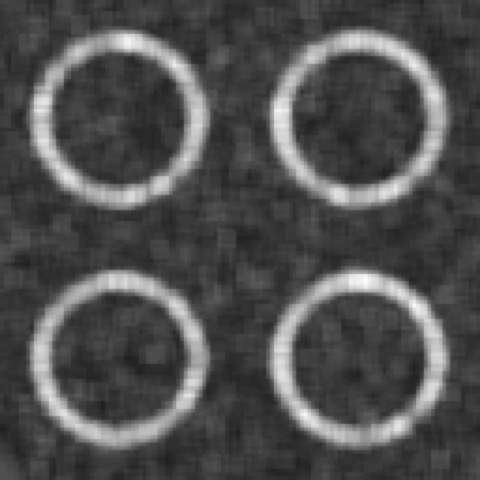
\includegraphics[width=\textwidth/4]{blur0.png}
    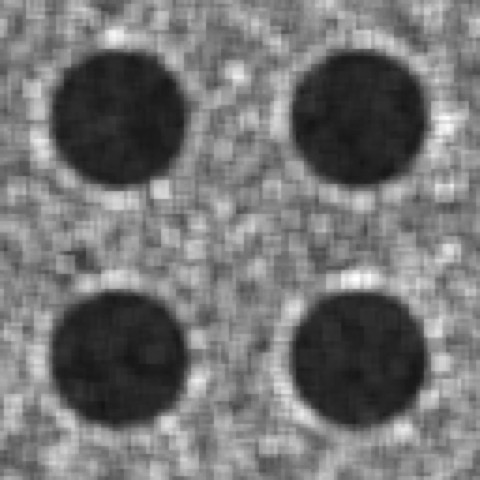
\includegraphics[width=\textwidth/4]{blur1.png}
    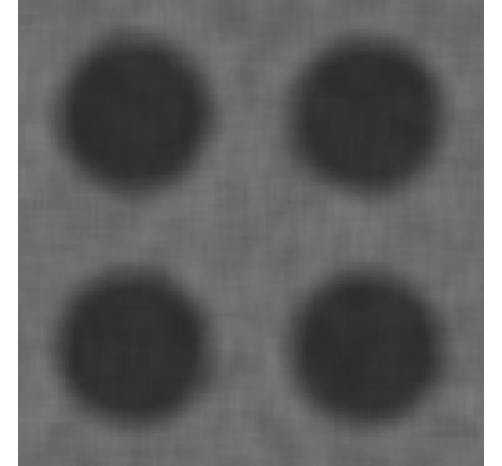
\includegraphics[width=\textwidth/4]{blur2.png}
    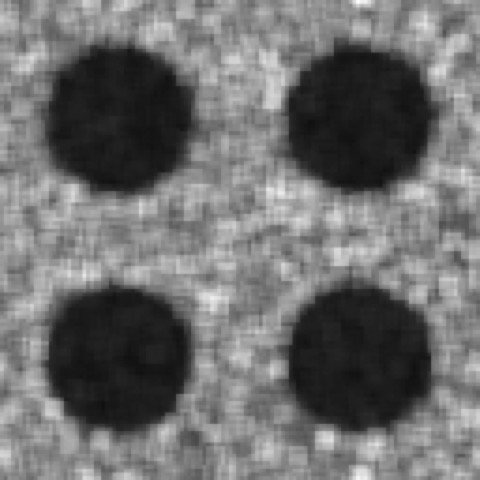
\includegraphics[width=\textwidth/4]{blur3.png}
    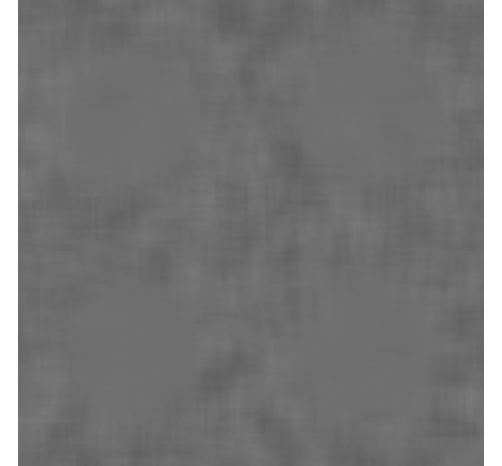
\includegraphics[width=\textwidth/4]{blur4.png}
    \caption{Result of rdfMoyenneImage() function}
    \label{fig-blur-images}
\end{figure}

\clearpage

\paragraph{}
Afterwards, we just follow the formula for the standard deviation for each pixel.
Observation: the image is normalised to have values between $0$ and $1$, since we're working with gray values.

\begin{lstlisting}[language=R, caption=Calculating a pixel's average value]
    # Ecart type normalise des voisinages carres d'une image
    rdfTextureEcartType <- function (image, taille) {
        # carre de l'image moins sa moyenne
        carre = (image - rdfMoyenneImage (image, taille)) ^ 2
        # ecart type
        ecart = sqrt (rdfMoyenneImage (carre, taille))
        # normalise pour maximum a 1
        ecart / max (ecart)
    }
\end{lstlisting}

\subsection{Histograms of texture levels}
Applying the methods above (neighbourhood size=$2$), we can build the following histograms of texture levels:
\begin{figure}[h]
    \centering
    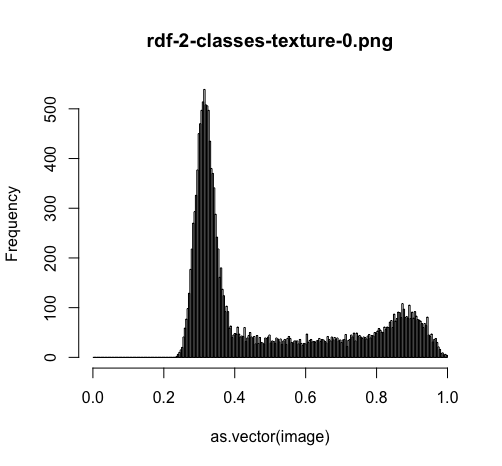
\includegraphics[width=\textwidth/3-10pt]{texture_levels_0.png}
    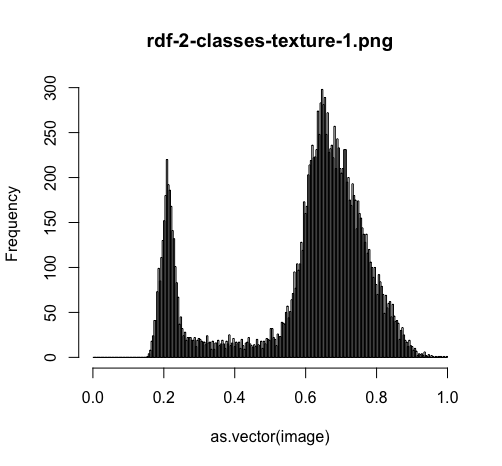
\includegraphics[width=\textwidth/3-10pt]{texture_levels_1.png}
    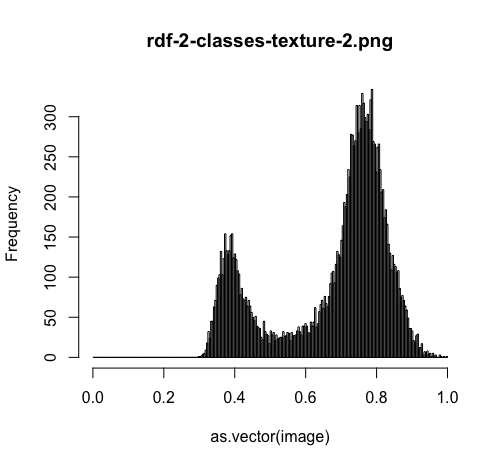
\includegraphics[width=\textwidth/3-10pt]{texture_levels_2.png}
    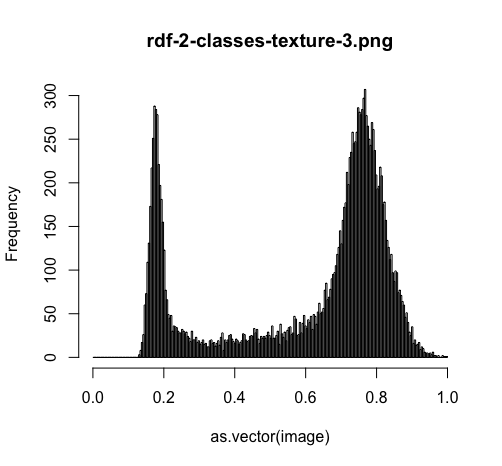
\includegraphics[width=\textwidth/3-10pt]{texture_levels_3.png}
    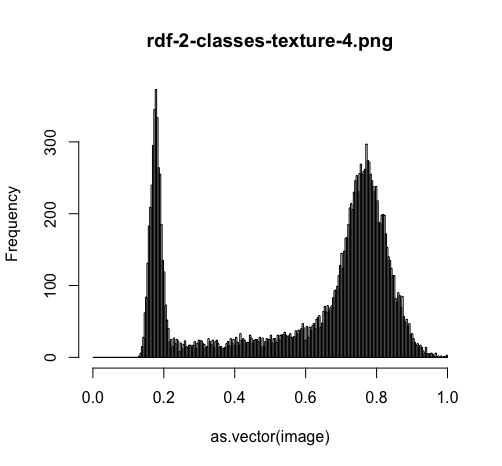
\includegraphics[width=\textwidth/3-10pt]{texture_levels_4.png}
    \caption{Histograms of gray values for each texture}
    \label{}
\end{figure}

\clearpage

An interesting observation is that we now have a ``valley'' for each texture, even for the noisy ones.
Next, we can use the same ``thresholding'' method as in our previous experiment \ref{experiment-thresholding}, but applied on the images obtained from \emph{rdfTextureEcartType()}.
\begin{figure}[h]
    \centering
    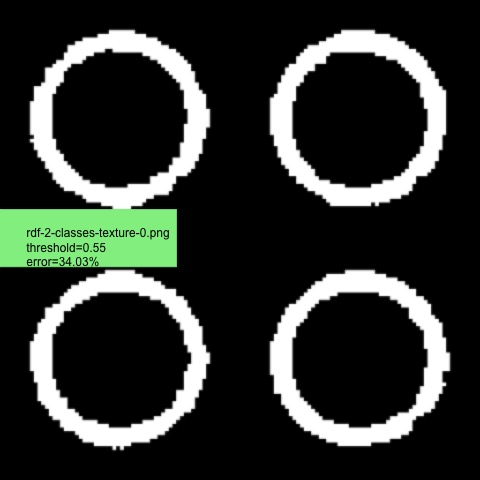
\includegraphics[width=\textwidth/3]{texture_thresholding_0.png}
    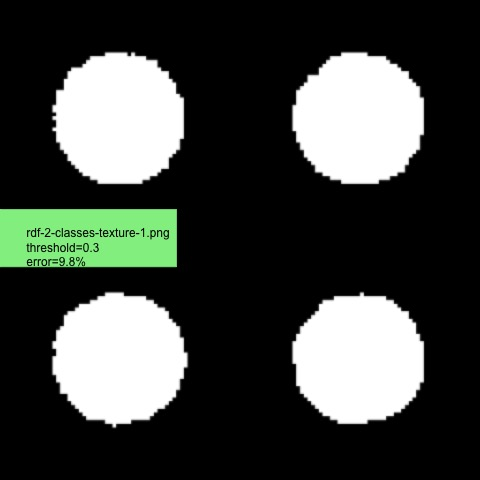
\includegraphics[width=\textwidth/3]{texture_thresholding_1.png}
    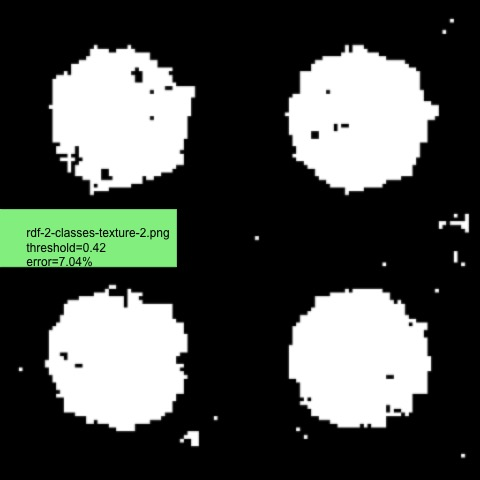
\includegraphics[width=\textwidth/3]{texture_thresholding_2.png}
    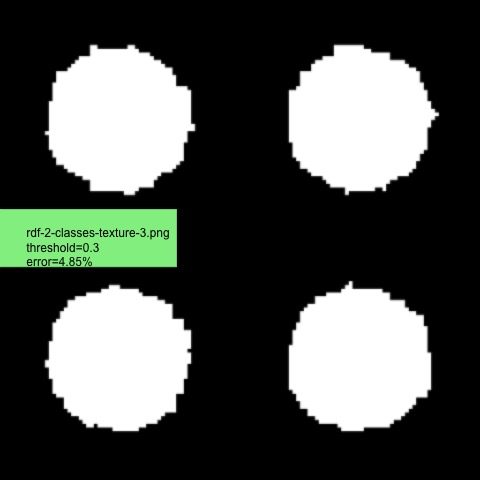
\includegraphics[width=\textwidth/3]{texture_thresholding_3.png}
    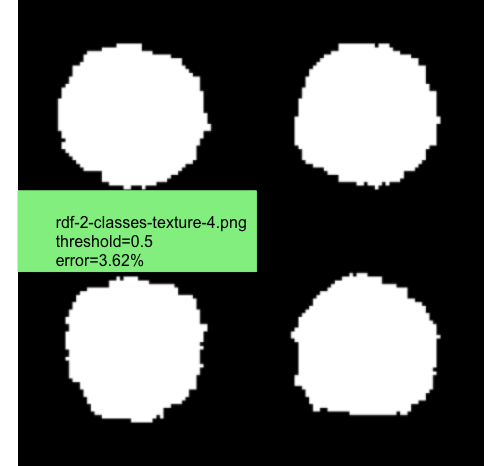
\includegraphics[width=\textwidth/3]{texture_thresholding_4.png}
    \caption{Thresholding based on texture}
\end{figure}

\paragraph{}
Our biggest win here, using texture levels, is that for the last 2 textures, the segmentation works much better, due to the ``mathematical blur'' we applied by calculating the average gray values.
However, this is still far from perfect, especially for the first texture, where our segmentation resulted in... donuts.
\paragraph{}
As a conclusion for this experiment, it seems like what ``gray thresholding'' does bad, ``texture thresholding'' does good and viceversa.
Given this, it might be a good idea to try and combine the two methods.

\clearpage

\section{Combining gray and texture levels}
\subsection{Conjoint Histograms}
\paragraph{}
A useful tool when working with images are \emph{conjoint histograms}: \cite{wiki_conjoint_histograms}
These help us analyse the difference between images.
We can create these histograms by using the original gray images and the ones we derived using the standard deviation. \ref{fig-blur-images}

\begin{lstlisting}[language=R, caption=Calculating conjoint histograms]
    # Calcul de l'histogramme 2D (log + normalise) de deux images
    rdfCalculeHistogramme2D <- function (image1, bins1, image2, bins2) {
        # Bins dans les deux images
        indices1 = findInterval (image1, seq (0, 1, 1 / bins1))
        indices2 = findInterval (image2, seq (0, 1, 1 / bins2))
        # Tableau de contingence
        counts <- table (indices1, indices2)
        # Extension en tableau 2D incluant les valeurs nulles
        liste <- as.data.frame (counts)
        h2d <- array (0, c (bins1, bins2))
        h2d[cbind (liste[,1], liste[,2])] <- liste[,3]
        # Passage en log
        h2d <- log (1 + h2d)
        # normalise pour maximum a 1
        as.Image (h2d / max (h2d))
    }
\end{lstlisting}

\paragraph{}
The \emph{findInterval()} function assigns each image pixel to its corresponding bin in the context of the single dimension histogram.
In our case, the number of bins will be $256$ for both.
Afterwards, the \emph{table()} function helps us build a \emph{contingency table} that we can use to build our resulted gray image. \cite{r_documentation}
\begin{figure}[h]
    \centering
    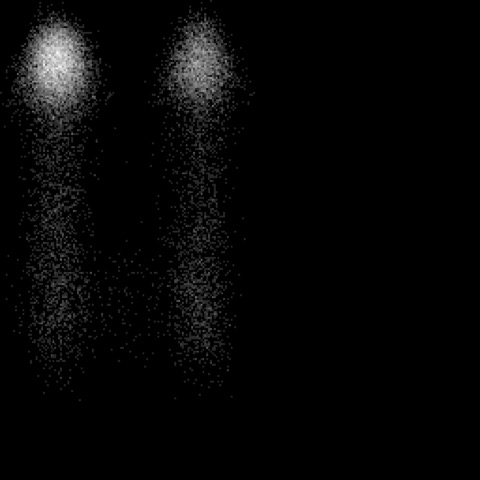
\includegraphics[width=\textwidth/3 - 10pt]{conjoint_0.png}
    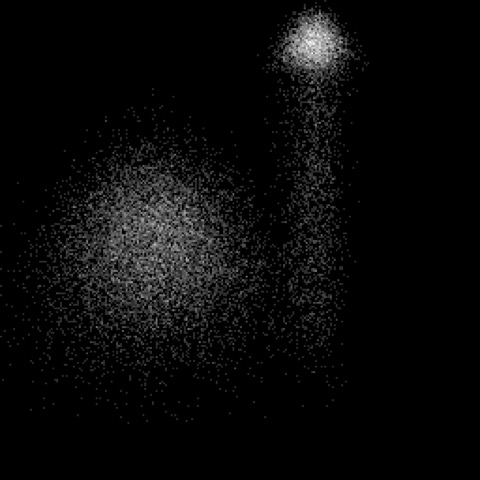
\includegraphics[width=\textwidth/3 - 10pt]{conjoint_1.png}
    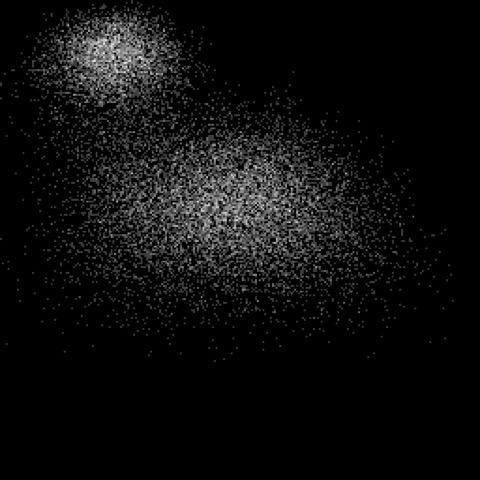
\includegraphics[width=\textwidth/3 - 10pt]{conjoint_2.png}
    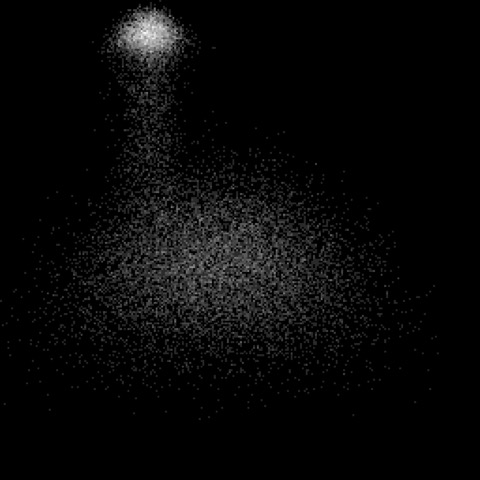
\includegraphics[width=\textwidth/3 - 10pt]{conjoint_3.png}
    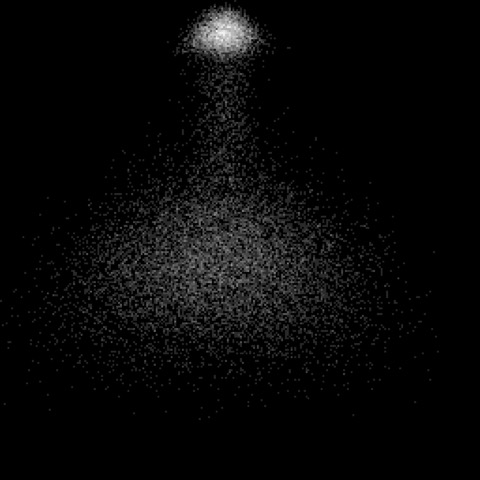
\includegraphics[width=\textwidth/3 - 10pt]{conjoint_4.png}
    \caption{Conjoint histograms for the textures}
\end{figure}

\paragraph{}
Our goal right now is to combine the two image attributes described above (the gray and the texture levels) to properly do the binary segmentation.
We can build a third gray image on which we will apply the thresholding method we described earlier.
For the third image, each pixel will have the following value:
\label{eq-linear-combination}
$$C_{ij} = a * G_{ij} + b * T_{ij}$$
where $C$ is our resulted image, $G$ is our gray image and $T$ our texture image.

\paragraph{}
Afterwards, we can normalise this image $C_{ij} = C_{ij}/\max(C)$ to obtain a gray one in which we can analyse the gray values histogram.
Looking at that histogram, we'll choose the threshold and finally do the binary segmentation.

\subsection{Finding the linear combination between $G$ and $T$}
\paragraph{}
In the equation above \ref{eq-linear-combination}, $a$ and $b$ correspond to the parameters of a line equation.
The line that those parameters represent may be the line that best separates the ``conglomerations'' of white pixels in our conjoint histogram.

\begin{figure}[h]
    \centering
    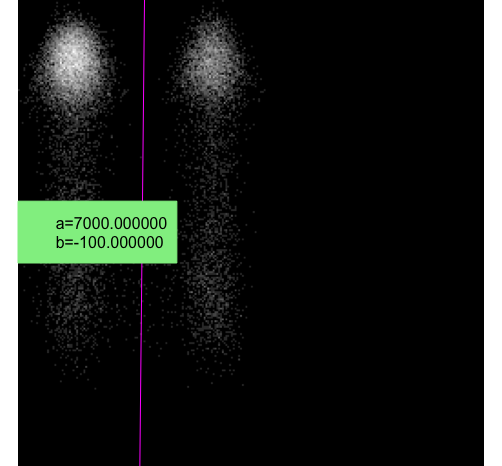
\includegraphics[width=\textwidth/3 - 10pt]{conjoint_line_0.png}
    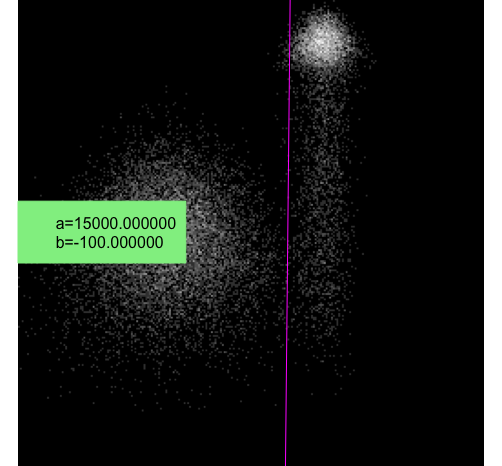
\includegraphics[width=\textwidth/3 - 10pt]{conjoint_line_1.png}
    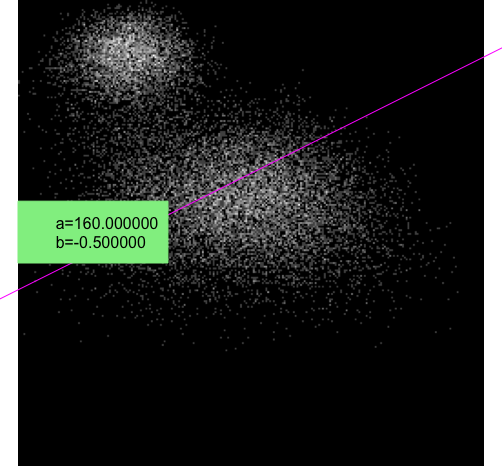
\includegraphics[width=\textwidth/3 - 10pt]{conjoint_line_2.png}
    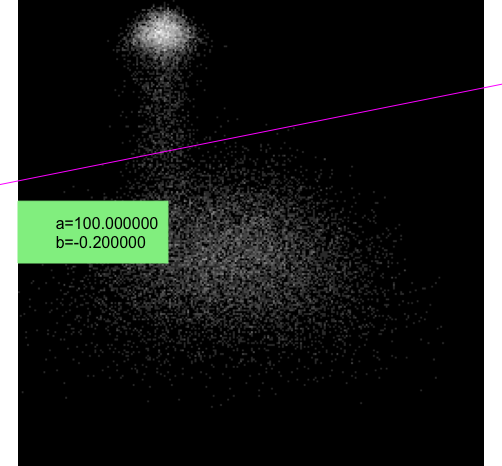
\includegraphics[width=\textwidth/3 - 10pt]{conjoint_line_3.png}
    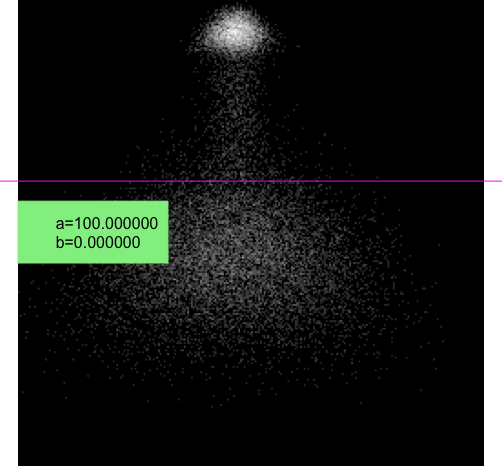
\includegraphics[width=\textwidth/3 - 10pt]{conjoint_line_4.png}
    \caption{Separating the attributes with a linear equation}
    \label{}
\end{figure}


\paragraph{}
Observation: The values for $a$ and $b$ were chosen ``by hand''. This won't result in the best results, but still useful to draw some conclusions.

\paragraph{}
After finding some satisfying values for $a$ and $b$, we can try and build our final grayscale images on which we'll apply a binary threshold based on the histograms for the gray values.

\begin{figure}[h]
    \centering
    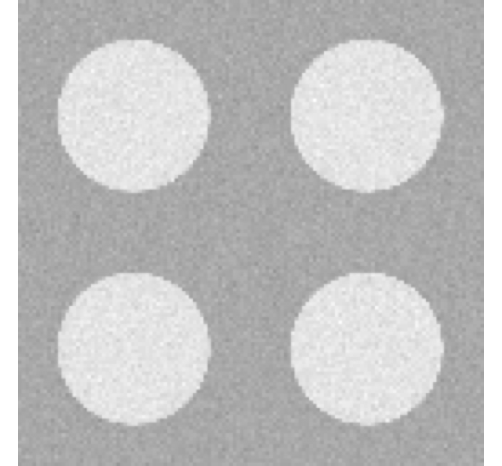
\includegraphics[width=\textwidth/3 - 10pt]{final_image_0.png}
    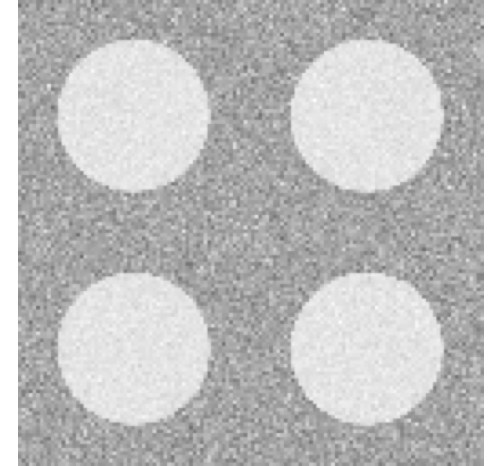
\includegraphics[width=\textwidth/3 - 10pt]{final_image_1.png}
    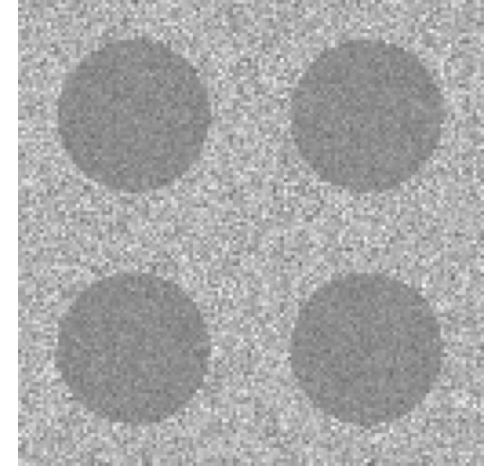
\includegraphics[width=\textwidth/3 - 10pt]{final_image_2.png}
    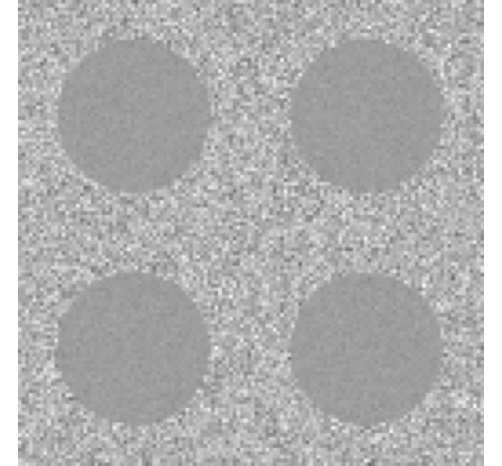
\includegraphics[width=\textwidth/3 - 10pt]{final_image_3.png}
    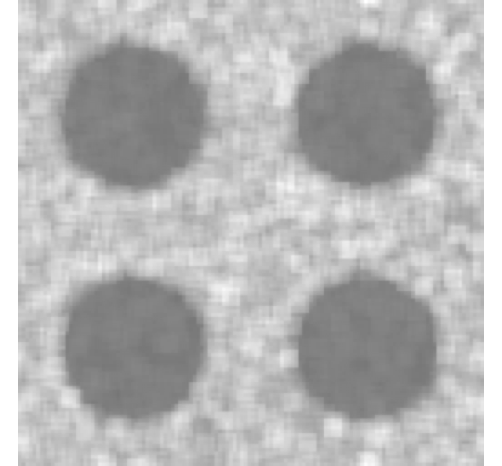
\includegraphics[width=\textwidth/3 - 10pt]{final_image_4.png}
    \caption{Final gray images}
    \label{}
\end{figure}

\begin{figure}[h]
    \centering
    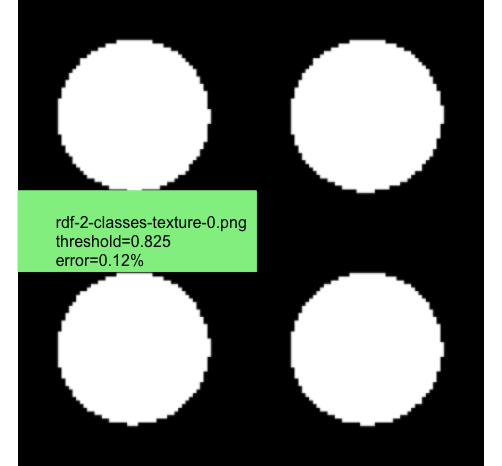
\includegraphics[width=\textwidth/3 - 10pt]{final_segmentation_0.png}
    \includegraphics[width=\textwidth/3 - 10pt]{final_segmentation_1.png}
    \includegraphics[width=\textwidth/3 - 10pt]{final_segmentation_2.png}
    \includegraphics[width=\textwidth/3 - 10pt]{final_segmentation_3.png}
    \includegraphics[width=\textwidth/3 - 10pt]{final_segmentation_4.png}
    \caption{Binary segmentation on the final images}
    \label{}
\end{figure}